\RequirePackage{atbegshi}
\documentclass[compress,aspectratio=169]{beamer}\usepackage[]{graphicx}\usepackage[]{color}
% maxwidth is the original width if it is less than linewidth
% otherwise use linewidth (to make sure the graphics do not exceed the margin)
\makeatletter
\def\maxwidth{ %
  \ifdim\Gin@nat@width>\linewidth
    \linewidth
  \else
    \Gin@nat@width
  \fi
}
\makeatother

\definecolor{fgcolor}{rgb}{0.345, 0.345, 0.345}
\newcommand{\hlnum}[1]{\textcolor[rgb]{0.686,0.059,0.569}{#1}}%
\newcommand{\hlstr}[1]{\textcolor[rgb]{0.192,0.494,0.8}{#1}}%
\newcommand{\hlcom}[1]{\textcolor[rgb]{0.678,0.584,0.686}{\textit{#1}}}%
\newcommand{\hlopt}[1]{\textcolor[rgb]{0,0,0}{#1}}%
\newcommand{\hlstd}[1]{\textcolor[rgb]{0.345,0.345,0.345}{#1}}%
\newcommand{\hlkwa}[1]{\textcolor[rgb]{0.161,0.373,0.58}{\textbf{#1}}}%
\newcommand{\hlkwb}[1]{\textcolor[rgb]{0.69,0.353,0.396}{#1}}%
\newcommand{\hlkwc}[1]{\textcolor[rgb]{0.333,0.667,0.333}{#1}}%
\newcommand{\hlkwd}[1]{\textcolor[rgb]{0.737,0.353,0.396}{\textbf{#1}}}%
\let\hlipl\hlkwb

\usepackage{framed}
\makeatletter
\newenvironment{kframe}{%
 \def\at@end@of@kframe{}%
 \ifinner\ifhmode%
  \def\at@end@of@kframe{\end{minipage}}%
  \begin{minipage}{\columnwidth}%
 \fi\fi%
 \def\FrameCommand##1{\hskip\@totalleftmargin \hskip-\fboxsep
 \colorbox{shadecolor}{##1}\hskip-\fboxsep
     % There is no \\@totalrightmargin, so:
     \hskip-\linewidth \hskip-\@totalleftmargin \hskip\columnwidth}%
 \MakeFramed {\advance\hsize-\width
   \@totalleftmargin\z@ \linewidth\hsize
   \@setminipage}}%
 {\par\unskip\endMakeFramed%
 \at@end@of@kframe}
\makeatother

\definecolor{shadecolor}{rgb}{.97, .97, .97}
\definecolor{messagecolor}{rgb}{0, 0, 0}
\definecolor{warningcolor}{rgb}{1, 0, 1}
\definecolor{errorcolor}{rgb}{1, 0, 0}
\newenvironment{knitrout}{}{} % an empty environment to be redefined in TeX

\usepackage{alltt} % aspectratio=169
%\usepackage[svgnames]{xcolor}

% % % % % % % % % % % % % % %
%             MY PACKAGES 
% % % % % % % % % % % % % % %
\usepackage{graphicx}       % Use pdf, png, jpg, or eps with pdflatex; use eps in DVI mode
\usepackage{dcolumn} % this pack is neccesary to build nicer columns with texreg--dont remove it.
\usepackage[export]{adjustbox}

\usepackage{amssymb}
\usepackage{amsmath}  
%\usepackage{tipx}
%\usepackage{tikz}
%\usetikzlibrary{arrows,shapes,decorations.pathmorphing,backgrounds,positioning,fit,petri}
\usepackage{rotating}
%\usepackage{scalerel} % for inline images
\usepackage{import}
%\usepackage{times}
\usepackage{array}
\usepackage{tabularx}
%\usepackage{booktabs}
%\usepackage{textcomp}
\usepackage{float}
%\usepackage{setspace}      % \doublespacing \singlespacing \onehalfspacing %doble espacio
%\label{x:y}                          %ocupar para autoref.
%\autoref{x:y}                        %ocupar para autoref.
%\usepackage{nopageno}      %desactivar para p�ginas
\usepackage{pifont}
%\usepackage{color,xcolor,ucs}
%\usepackage{marvosym} %faces
\usepackage{hyperref}
\usepackage{multirow}


\usepackage{listings}
\usepackage{color}
\definecolor{dkgreen}{rgb}{0,0.6,0}
\definecolor{gray}{rgb}{0.5,0.5,0.5}
\definecolor{mauve}{rgb}{0.58,0,0.82}
\lstset{ %
  language=R,                     % the language of the code
  basicstyle=\TINY,           % the size of the fonts that are used for the code
  numbers=left,                   % where to put the line-numbers
  numberstyle=\tiny\color{gray},  % the style that is used for the line-numbers
  stepnumber=1,                   % the step between two line-numbers. If it's 1, each line
                                  % will be numbered
  numbersep=5pt,                  % how far the line-numbers are from the code
  backgroundcolor=\color{white},  % choose the background color. You must add \usepackage{color}
  showspaces=false,               % show spaces adding particular underscores
  showstringspaces=false,         % underline spaces within strings
  showtabs=false,                 % show tabs within strings adding particular underscores
  frame=single,                   % adds a frame around the code
  rulecolor=\color{black},        % if not set, the frame-color may be changed on line-breaks within not-black text (e.g. commens (green here))
  tabsize=1,                      % sets default tabsize to 2 spaces
  captionpos=b,                   % sets the caption-position to bottom
  breaklines=true,                % sets automatic line breaking
  breakatwhitespace=false,        % sets if automatic breaks should only happen at whitespace
  title=\lstname,                 % show the filename of files included with \lstinputlisting;
                                  % also try caption instead of title
  keywordstyle=\color{blue},      % keyword style
  commentstyle=\color{dkgreen},   % comment style
  stringstyle=\color{mauve},      % string literal style
  escapeinside={\%*}{*)},         % if you want to add a comment within your code
  morekeywords={*,...}            % if you want to add more keywords to the set
} 

% % % % % % % % % % % % % % %
%           PACKAGE CUSTOMIZATION
% % % % % % % % % % % % % % %

% GENERAL CUSTOMIZATION
\usepackage[math]{iwona}% font
\usetheme{Singapore}  % template I should use
%\usetheme{Szeged}  % alternative template
\usecolortheme{rose}  % color template
\makeatletter     % to show subsection/section title (1/3)
\beamer@theme@subsectiontrue % to show subsection/section title (2/3)
\makeatother      % to show subsection/section title (3/3)



% THIS BELOW IS TO MAKE NAVIGATION DOTS MARKED DURING PRESENTATION
\makeatletter
\def\slideentry#1#2#3#4#5#6{%
  %section number, subsection number, slide number, first/last frame, page number, part number
  \ifnum#6=\c@part\ifnum#2>0\ifnum#3>0%
    \ifbeamer@compress%
      \advance\beamer@xpos by1\relax%
    \else%
      \beamer@xpos=#3\relax%
      \beamer@ypos=#2\relax%
    \fi%
  \hbox to 0pt{%
    \beamer@tempdim=-\beamer@vboxoffset%
    \advance\beamer@tempdim by-\beamer@boxsize%
    \multiply\beamer@tempdim by\beamer@ypos%
    \advance\beamer@tempdim by -.05cm%
    \raise\beamer@tempdim\hbox{%
      \beamer@tempdim=\beamer@boxsize%
      \multiply\beamer@tempdim by\beamer@xpos%
      \advance\beamer@tempdim by -\beamer@boxsize%
      \advance\beamer@tempdim by 1pt%
      \kern\beamer@tempdim
      \global\beamer@section@min@dim\beamer@tempdim
      \hbox{\beamer@link(#4){%
          \usebeamerfont{mini frame}%
          \ifnum\c@section>#1%
            %\usebeamercolor[fg]{mini frame}%
            %\usebeamertemplate{mini frame}%
            \usebeamercolor{mini frame}%
            \usebeamertemplate{mini frame in other subsection}%
          \else%
            \ifnum\c@section=#1%
              \ifnum\c@subsection>#2%
                \usebeamercolor[fg]{mini frame}%
                \usebeamertemplate{mini frame}%
              \else%
                \ifnum\c@subsection=#2%
                  \usebeamercolor[fg]{mini frame}%
                  \ifnum\c@subsectionslide<#3%
                    \usebeamertemplate{mini frame in current subsection}%
                  \else%
                    \usebeamertemplate{mini frame}%
                  \fi%
                \else%
                  \usebeamercolor{mini frame}%
                  \usebeamertemplate{mini frame in other subsection}%
                \fi%
              \fi%
            \else%
              \usebeamercolor{mini frame}%
              \usebeamertemplate{mini frame in other subsection}%
            \fi%
          \fi%
        }}}\hskip-10cm plus 1fil%
  }\fi\fi%
  \else%
  \fakeslideentry{#1}{#2}{#3}{#4}{#5}{#6}%
  \fi\ignorespaces
  }
\makeatother


% % % % % % % % % % % % % % %
%       To show the TITLE at the Bottom of each slide
% % % % % % % % % % % % % % %

\beamertemplatenavigationsymbolsempty 
\makeatletter
\setbeamertemplate{footline}
{
\leavevmode%
\hbox{%
\begin{beamercolorbox}[wd=1\paperwidth,ht=2.25ex,dp=2ex,center]{title in head/foot}%
\usebeamerfont{title in head/foot}\insertshorttitle
\end{beamercolorbox}%
\begin{beamercolorbox}[wd=1
\paperwidth,ht=2.25ex,dp=2ex,center]{date in head/foot}%
\end{beamercolorbox}}%
}
\makeatother



% to switch off navigation bullets
%% using \miniframeson or \miniframesoff
\makeatletter
\let\beamer@writeslidentry@miniframeson=\beamer@writeslidentry
\def\beamer@writeslidentry@miniframesoff{%
  \expandafter\beamer@ifempty\expandafter{\beamer@framestartpage}{}% does not happen normally
  {%else
    % removed \addtocontents commands
    \clearpage\beamer@notesactions%
  }
}
\newcommand*{\miniframeson}{\let\beamer@writeslidentry=\beamer@writeslidentry@miniframeson}
\newcommand*{\miniframesoff}{\let\beamer@writeslidentry=\beamer@writeslidentry@miniframesoff}
\makeatother

% Image full size: use 
%%\begin{frame}
  %%\fullsizegraphic{monogram.jpg}
%%\end{frame}
\newcommand<>{\fullsizegraphic}[1]{
  \begin{textblock*}{0cm}(-1cm,-3.78cm)
  \includegraphics[width=\paperwidth]{#1}
  \end{textblock*}
}


% hyperlinks
\hypersetup{colorlinks,
            urlcolor=[rgb]{0.01, 0.28, 1.0},
            linkcolor=[rgb]{0.01, 0.28, 1.0}}


% % % % % % % % % % % % % % %
%           DOCUMENT ID
% % % % % % % % % % % % % % %

\title{\input{title.txt}\unskip}

\author[shortname]{H\'ector Bahamonde \textsuperscript{1} \and Andrea Canales \inst{1}}
\institute[shortinst]{\textsuperscript{1} O$'$Higgins University}
\date{\today}

%to to see shadows of previous blocks
%\setbeamercovered{dynamic}
\IfFileExists{upquote.sty}{\usepackage{upquote}}{}
\begin{document}







% % % % % % % % % % % % % % %
%           CONTENT
% % % % % % % % % % % % % % %

%% title frame
\begin{frame}
\titlepage
\end{frame}


\section{Motivation}
\subsection{Motivation}

\begin{frame}{Motivation: Vote-Buying Literature Forgets About Vote-Sellers}

  \begin{itemize}
    \item The clientelism literature has focused primarily on vote-\emph{buying} (parties buying votes in exchange of electoral support).
    \item Unfortunately, we are rather ignorants about vote-\emph{sellers}: Who are they?
    \item Moreover, we do not know the micro-dynamics of the transaction itself.
    \item {\bf Supply and demand story}: Do parties target likely voters? Why? At what price? Under what conditions sellers their votes?
  \end{itemize}
\end{frame}



\section{Formal Model}
\subsection{Formal Model}

\begin{frame}{Formal Model}

\end{frame}




















































































































































\section{Experimental Design}


\subsection{Experimental Design}



\begin{frame}{Experimental Design}

Parts:
  \begin{enumerate}
    \item Vote-buying: parties are first players (get out and buy votes, if needed).
    \item Vote-selling: voters are first players (get out and sell votes, if needed).
  \end{enumerate}

For both parts (VB, VS), the following stages:
  \begin{enumerate}
    \item Random assignments: role (P, V), ``ideology,'' ``party endowments.''
    \item buying/selling {\bf offers}.
    \item buying/selling choice {\bf choices}.
    \item Election.
  \end{enumerate}

\end{frame}



\begin{frame}{Experimental Flow}
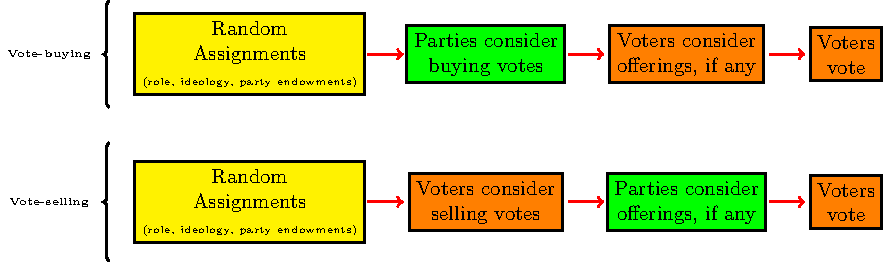
\includegraphics[scale=1, center]{Experimental_Flow_Figure.pdf}
\end{frame}


\begin{frame}{Caveats}
 \begin{itemize}
    \item Ideology: voters ``lean'' towards a party based on the amount of points received if party wins the election.\\
    \scriptsize{{\bf Not really ``ideology.''}}
    \item Party endowments: while both parties (A, B) receive the same amount, the \underline{relative} purchasing power of them is randomized indirectly (by randomizing the spatial party-voter distance). {\color{red}{\bf Parties face different vote-buying costs depending on party-voter distance.}}
    \item {\bf Relative importance of voter is randomized}. Voters are told they represent $\frac{1}{3}$ or $\frac{1}{5}$of voters. It mimics ``block voting.'' This is public knowledge.
  \end{itemize}
\end{frame}




\begin{frame}{Comparative Statics: Ideology}
 \begin{itemize}
    \item Downsian paradigm is unidimensional: left-right continuum (policy-oriented).
    \item We add some more complexity: non-policy factors (vote-selling is not policy-oriented).
    \item Research question: {\bf What's the tipping point at which voters stop caring about ideology, and start selling their votes?}
  \end{itemize}
\end{frame}



\begin{frame}{Comparative Statics: Competitiveness}
 \begin{itemize}
    \item Competitive authoritarian regimes (Levitsky and Way 2010) survive not due to electoral fraud.
    \item They survive because of the incumbent's capacity to mobilize a large mass of supporters, discouraging likely opposers (Magaloni 2008).
    \item Research question: 
      \begin{enumerate}
        \item {\bf At which point do likely opposers feel \underline{encouraged} and start buying votes?}
        \item {\bf At which point do likely opposers feel \underline{discouraged} and abandon the electoral race, not buying votes?}
      \end{enumerate}
  \end{itemize}
\end{frame}



\begin{frame}{Comparative Statics: Endowments}
 \begin{itemize}
    \item Literature won't give a definitive answer: Parties with more resources buy votes at higher prices (Bahamonde 2018) or not (Szwarcberg (2013).
    \item Research question: {\bf Do parties with more resources engage in vote-buying?}
    \item \scriptsize{\emph{Remember caveat: not ``really'' randomized. Proxy.}}
  \end{itemize}
\end{frame}


\begin{frame}{Comparative Statics: Targeting}
 \begin{itemize}
    \item Literature won't give a definitive answer: since it's cheaper, parties target own supporters (Cox and McCubbins), or parties target unlikely voters, otherwise, it's a waste (Stokes).
    \item Research question: {\bf Who do political parties target? Swing voters or core supporters?}
  \end{itemize}
\end{frame}


\begin{frame}{Comparative Statics: Sequence}
 \begin{itemize}
    \item Does being the first one in making an offer (buying/selling votes) matter? When? How?
  \end{itemize}
\end{frame}



\end{document}

